\documentclass{article}
\usepackage{graphicx}
\usepackage{fullpage}
\usepackage{amsmath}

\title{Übungsblatt 10}
\author{Tobias Baake (247074), Dylan Ellinger (247316), Nikiforos Tompoulidis (247714)}
\begin{document}
\maketitle

\section{Bresenham}
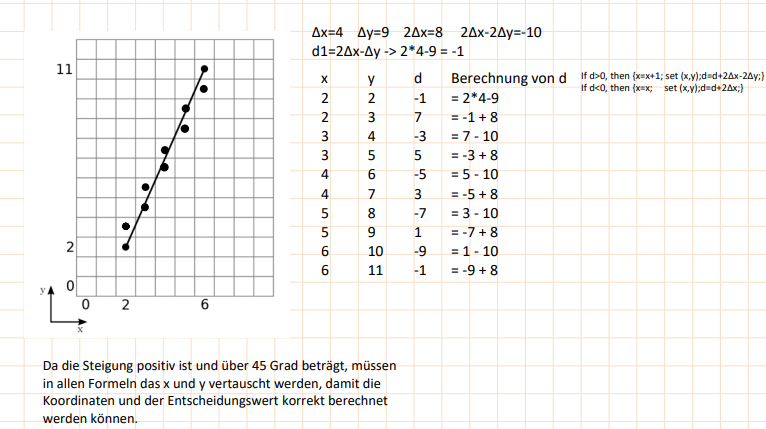
\includegraphics[width=370pt]{./files/Übung11.1.png}

\section{BSP-Bäume}
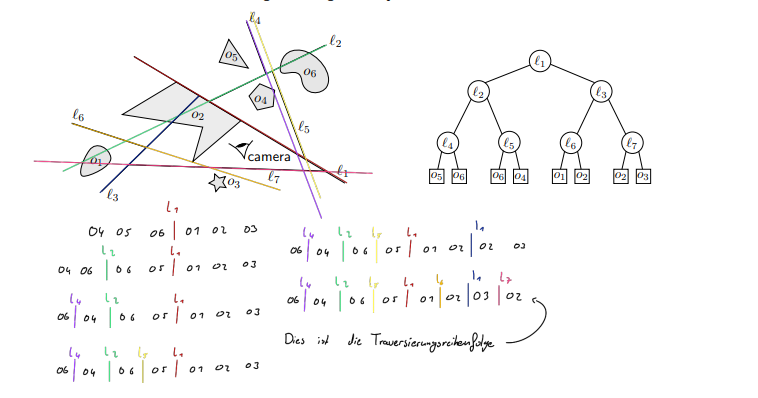
\includegraphics[width=400pt]{./files/Übung11.2.png}

\section{Potentially Visible Sets}
\subsection*{Ausgangszelle H}
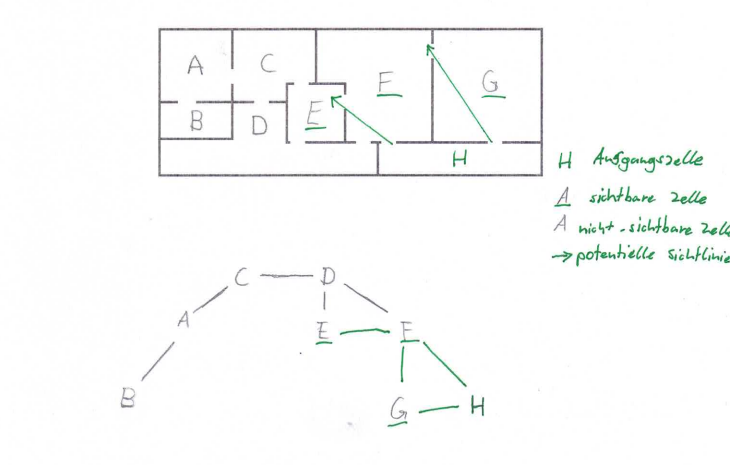
\includegraphics[width=400pt]{./files/Übung11.3.1.png}
\subsection*{Ausgangszelle D}
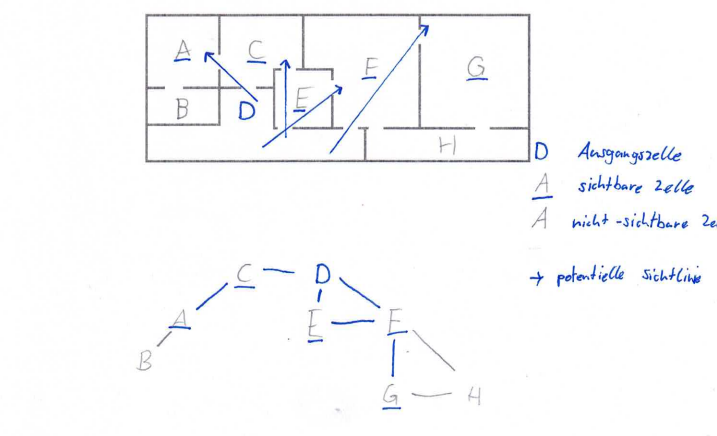
\includegraphics[width=400pt]{./files/Übung11.3.2.png}

\section{Bonus}

\includegraphics[width=140pt]{./files/Übung11.4.1.png}
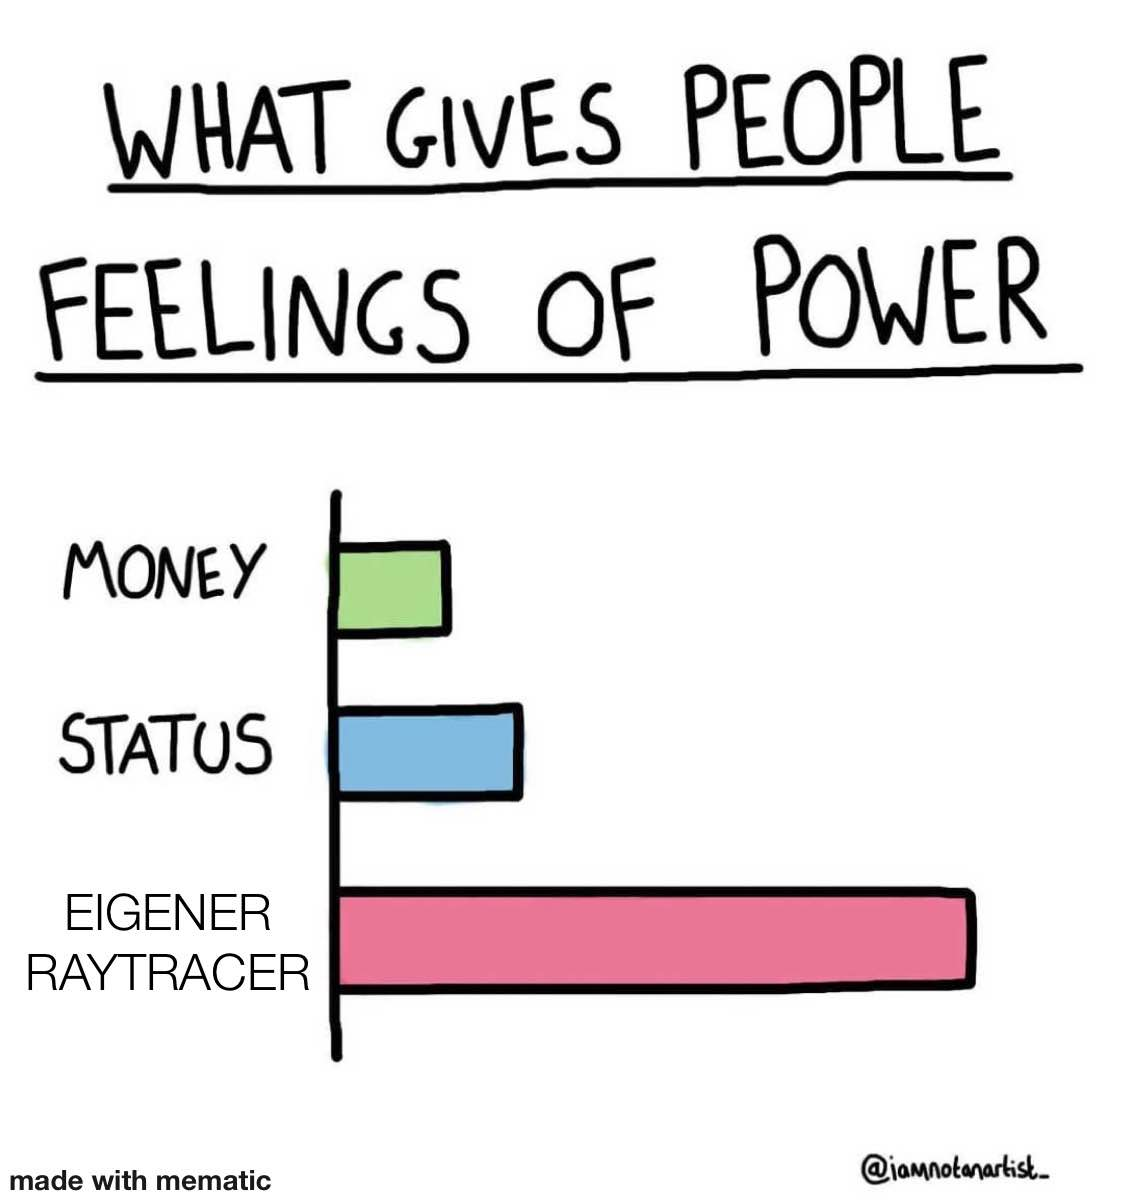
\includegraphics[width=140pt]{./files/Übung11.4.2.png}

\includegraphics[width=140pt]{./files/Übung11.4.3.png}
\end{document}